%\documentclass[14pt]{matmex-diploma-custom}
%\hyphenation{Ge-ne-ra-lised}
\newtheorem{mydef}{Определение}
%\tolerance=1
\emergencystretch=\maxdimen
%\hyphenpenalty=10000
%\hbadness=10000



\title{Поддержка расширенных контекстно-свободных грамматик 
	в алгоритме синтаксического анализа Generalised LL}

\titlerunning{Поддержка расширенных контекстно-свободных грамматик 
	в GLL}

\author{Горохов Артем Владимирович}

\authorrunning{А.В.Горохов}

\tocauthor{А.В.Горохов}
\institute{Санкт-Петербургский государственный университет\\
	\email{gorohov.art@gmail.com}}

\maketitle

\begin{abstract}
	Для автоматизации разработки синтаксических анализаторов часто используют генераторы, строящие анализаторы на основе спецификации языка.
	Обычно спецификация описывается неоднозначной грамматикой в расширенной форме Бэкуса-Наура (EBNF), которую не могут обрабатывать большинство инструментов без преобразования
	к форме Бэкуса-Наура (BNF).	Существующие подходы анализа EBNF без преобразования к BNF не способны обрабатывать неоднозначные грамматики. С другой стороны, алгоритм Generalized LL (GLL) допускает произвольные контекстно-свободные грамматики и достигает	высокой производительности, но не способен обрабатывать EBNF грамматики. 
	В данной работе описана модификация GLL алгоритма для обработки расширенных контекстно-свободных грамматик,
	эта форма родственна EBNF. Так же показано, что предложенный подход повышает производительность анализа по сравнению с алгоритмами использующими преобразование грамматик.
\end{abstract}


\section*{Введение}

Статический анализ --- это анализ программного кода без его исполнения. Он производится после синтаксического анализа на основе грамматики,
описывающей синтаксис языка.
%над структурным представлением кода, получаемым в результате синтаксического анализа. 
Общеупотребимый способ описания синтаксиса языков программирования --- грамматики в расширенной форме Бэкуса-Наура (EBNF)~\cite{EBNFISO}.
С одной стороны, эта форма проста для понимания людей, с другой, достаточно формальна и допускает автоматизированное создание синтаксических анализаторов.
Примером могут служить спецификации языков $C$, $C++$, $Java$ и т.д. 

Проблема в том, что существующие генераторы анализаторов, такие как ANTLR~\cite{ANTLRa}, Bison~\cite{Bison}, преобразуют грамматики в форму EBNF
для упрощения их структуры. В результате этого, представление кода строится на основе грамматики, отличной от заданной,
что затрудняет обработку результатов анализа. С другой стороны, производительность таких алгоритмов анализа,
как Generalised LL (GLL)~\cite{scott2010gll}
зависит от структуры грамматики, а её упрощение часто ведёт к избыточности представления, что отрицательно сказывается на производительности.

Алгоритм GLL показывает высокую производительность и способен работать с неоднозначными грамматиками. 
Предполагается, что поддержка в нём EBNF или родственных этой форме расширенных контекстно-свободных грамматик,
увеличит производительность анализа для некоторых грамматик.

% todo хочется дополнить
В данной работе предложен алгоритм синтаксического анализа, основанный на Generalised LL, для работы с расширенными
контекстно-свободными грамматиками без преобразований.
Показанно, что для некоторых грамматик алгоритм более производителен, чем существующие вариации GLL.
В разделе 1 представлен обзор предметной области и литературы. Далее в разделе 2 представлены необходимые изменения в Generalised LL алгоритме
и сопутствующих структурах данных. В разделе 3 описаны пути применения описанного алгоритма в задаче анализа регулярных множеств.
Эксперементальное сравнение полученного алгоритма с современными модификациями Generalised LL содержится в разделе 4.

\section{Обзор предметной области}
Заметим, что EBNF 
является стандартизированной формой для \textit{расширенных контекстно-свободных грамматик}.

\begin{mydef}
	Расширенная контекстно-свободная грамматика (ECFG)~\cite{ECFG} --- это кортеж $(N, \Sigma, P, S)$,
	где N и $\Sigma$ конечные множества нетерминалов и терминалов соответственно, 
	$S\in N$ является стартовым символом, а P (продукция) является отображением из N в
	регулярное выражение над алфавитом $N \cup \Sigma$.    
\end{mydef}

%ECFG широко используется в качестве входного формата для генераторов синтаксических анализаторов, 
%но классические алгоритмы синтаксического анализа часто требуют форму Бэкуса-Наура (BNF),
%в продукциях которой допускаются лишь последовательности из терминалов и нетерминалов. Таким образом 
%для работы генераторов анализаторов требуется преобразование в BNF.
%Возможно преобразование ECFG в BNF~\cite{ELL}, но оно приводит к увеличению
%размера грамматики и изменению её структуры: при трансформации добавляются новые
%нетерминалы. В результате синтаксический анализатор строит дерево вывода относительно
%преобразованной грамматики, и разработчику языка сложнее отлаживать грамматику 
%и использовать результат синтаксического анализа. Кроме того, увеличение размера грамматики 
%отрицательно сказывается на производительности анализа.

Существует широкий спектр методов анализа и алгоритмов~\cite{AttributedELL,ELRR,
	ECFGparsing,ELLParser,ELL,ECFG,ELALR,ELRParsing}, предназначенных для обработки
ECFG. Детальный обзор результатов и задач в этой области представлены в работе~\cite{ECFG}.
Следует отметить, что большинство алгоритмов основано на методах
LL-анализа~\cite{ELLParser,AttributedELL,PredictiveECFG} и LR-анализа~\cite{ELRParsing,ELALR,ELRR},
но они работают только с ограниченными подклассами расширенных контекстно-свободных грамматик ---
LL(k), LR(k). Таким образом, нет решения для обработки произвольных (в том числе неоднозначных) ECFG-грамматик.

ECFG-грамматики широко используется в качестве входного формата для генераторов синтаксических анализаторов, 
но классические алгоритмы синтаксического анализа часто требуют форму Бэкуса-Наура (BNF),
в продукциях которой допускаются лишь последовательности из терминалов и нетерминалов.
Возможно преобразование грамматик ECFG в форму BNF \cite{ELL}, но оно приводит к увеличению
размера грамматики и изменению её структуры: при трансформации добавляются новые
нетерминалы. В результате синтаксический анализатор строит дерево вывода относительно
преобразованной грамматики, что затрудняет обработку результата анализа.

В настоящее время алгоритмы на основе LL(1)-анализа представляются
наиболее практичными и обеспечивают лучшую диагностику ошибок по сравнению с LR-анализом, так как являются низходящими. 
Но некоторые грамматики не являются LL(k) (для любого k) и не могут быть использованы в LL(k) анализаторах.
Другие проблемы для инструментов на основе LL --- леворекурсивные грамматики и неоднозначности в грамматике, 
которые, вместе с предыдущим недостатком, усложняют создание анализаторов. 
Алгоритм Generalised LL, предложенный в~\cite{scott2010gll}, решает 
все эти проблемы: он обрабатывает произвольные CFG, в том числе неоднозначные и леворекурсивные.
В общем случае временная и пространственная сложность GLL зависит кубически от 
размера входа. А для LL(1) грамматик, он демонстрирует линейную временную и
пространственную сложность. Но он, как и другие современные алгоритмы, не допускает использования ECFG 
без предварительного преобразования к форме BNF.

Для увеличения производительности Generalised LL-алгоритма, была предложена поддержка 
лево-факторизованных грамматик в нём~\cite{scott2016structuring}.
Алгоритм GLL обрабатывает все возможные ветви разбора строки по заданной грамматике, 
эти ветви описываются так называемыми дескрипторами, которые состоят из позиций в грамматике и во входе,
корня построенного леса разбора и текущего узла стека. Из этого следует, что для уменьшения времени анализа и количества используемой памяти
можно снизить количество дескрипторов для обработки. Один из путей для достижения этого --- 
уменьшение размера грамматики (снижение количества различных позиций в ней).
Этого можно достичь факторизацией грамматики. Пример факторизации показан на рис.~\ref{fig:ExampleOfFactorization}:
из грамматики $G_0$ в процессе факторизации получена грамматика $G_0'$.
Этот пример рассмотрен в работе~\cite{scott2016structuring}, и доказано, что для некоторых грамматик факторизация 
существенно увеличивает производительность алгоритма GLL.
\begin{figure}
	\centering
	\subfloat[Исходная грамматика $G_0$]{
		$
		\begin{array}{rl}
		S::= a\ a\ b\ c\ d \ | \ a\ a\ c\ d \ | \ a\ a\ c\ e |\ a\ a
		\end{array}
		$
	}
	~
	\subfloat[Факторизованная грамматика $G_0'$]{
		$
		\begin{array}{rl}
		S::= a\ a\ ( b\ c\ d\ |\ c\ ( d\ |\ e )\ |\ \varepsilon \ )
		\end{array}
		$
	}
	\caption{Пример факторизации грамматики}
	\label{fig:ExampleOfFactorization}
\end{figure}

Одно из возможных применений обобщённого синтаксического анализа --- синтаксический анализ регулярных множеств.
Синтаксическим анализом регулярных множеств называют анализ строк, заданных всеми возможными путями в конечном автомате.
Такая задача возникает в различных областях одна из которых --- биоинформатика. В результате экспериментов 
получают данные о геномах организмов, которые представлены строками в конечном автомате (геномы это строки над алфавитом $\{A;C; G; T\}$).
Этот автомат называется метагеномной сборкой.

Существует множество подходов к анализу и идентификации геномов. Один из них --- поиск и сравнение участков таких структур как
16s рРНК, тРНК, так как по ним можно достаточно точно классифицировать организм, которому они принадлежат.
Существуют такие инструменты, как REAGO~\cite{reago} и HMMER~\cite{hmmer}, использующие скрытые цепи Маркова для поиска, 
Infernal~\cite{Infernal}, использующий ковариационные модели. Но они работают лишь с линейными цепочками генома ---
не объединёнными в конечный автомат, такое представление требует большого количества памяти и неэффективно.
С другой стороны, инструмент Xander~\cite{xander} использует композицию скрытых моделей Маркова и метагеномных сборок.
Изъян данного инструмента в существенно более низкой точности результата в сравнении с инструментами, использующими ковариационные модели.

Другой подход разрабатывается в лаборатории JetBrains СПбГУ.
Поиск производится непосредственно в метагеномной сборке по таким структурам как тРНК, 16s рРНК.
Эти структуры имеют некоторые общие свойства в строении, которые могут быть описаны
контекстно-свободной грамматикой~\cite{Anderson2013a}.
Таким образом, можно использовать синтаксический анализ регулярных множеств для поиска.
Этот подход описан в работе~\cite{ragozina}, основан на алгоритме синтаксического анализа Generalised LL и 
был реализован в рамках проекта YaccConstructor~\cite{YaccConstructor}. В нашей работе 
будут использоваться результаты и данные из работы~\cite{ragozina} для сравнения производительности полученного алгоритма.

\section{Использование Generalised LL для обработки ECFG}

В этом разделе описываются структуры и методы необходимые для использования расширенных контекстно-свободных грамматик 
в алгоритме синтаксического анализа Generalised LL, а так же необходимые изменения в алгоритме анализа.

\subsection{Представление ECFG}

Представление ECFG, наиболее подходящее для синтаксического анализа --- рекурсивные автоматы
(Recursive Automaton (RA)~\cite{tellier2006learning}.
\begin{mydef}
	Рекурсивный автомат $R$ это кортеж $(\Sigma, Q, S, F, \delta)$, где $\Sigma$
	--- конечное множество терминалов, $Q$ - конечное множество состояний, $S \in Q$ 
	--- начальное состояние, $F \subseteq Q$ --- множество конечных состояний,
	$\delta : Q \times (\Sigma \cup Q) \to Q$ --- функция перехода.
\end{mydef}
В рамках этой работы единственное различие между рекурсивным автоматом и общеизвестным
конечным автоматом (FSA) состоит в том, что переходы в RA обозначаются либо терминалом ($\Sigma$),
либо состоянием автомата ($Q$). Далее будем называть переходы помеченные элементами из
$Q$ \textit{нетерминальными переходами}, а терминалами --- \textit{терминальными переходами}.
Нетерминальный переход в состояние $q$ подразумевают построение вывода для некоторой подстроки начиная с текущей позиции во входе
по этому нетерминалу и последующий разбор оставшейся подстроки начиная с состояния $q$.

Заметим, что позиции грамматики эквивалентны состояниям автомата, которые 
строятся из правых частей продукций грамматики. Правые части продукций ECFG являются регулярными
выражениями над объединенным алфавитом терминалов и нетерминалов, поэтому построить по ним автомат можно использую общеизвестные алгоритмы.
Следующий алгоритма строит RA с минимальным числом состояний для заданной ECFG.
\begin{itemize}
	\item Построить конечный автомат, используя метод Томпсона~\cite{Thompson:1968:PTR:363347.363387} для правых
	частей продукций.
	\item Создать ассоциативный массив $M$ из каждого нетерминала в соответствующее начальное состояние автомата.
	Этот массив должен оставаться консистентным на протяжение всех следующих шагов.
	\item Преобразовать автоматы из предыдущего шага в детерминированные без 
	$\varepsilon$-переходов используя алгоритм, описанный в~\cite{aho1974design}.
	\item Минимизировать детерминированный автомат, используя, например, алгоритм
	Джона Хопкрофта~\cite{hopcroft1971n}.
	\item Заменить нетерминальные переходы переходами по, стартовым состояниям автоматов,
	соответствующим данным нетерминалам, используя массив $M$. Результат 
	этого шага --- искомый рекурсивный автомат. Также используем $M$
	для определения функции $\Delta : Q \to N$ где $N$ --- имя нетерминала.
\end{itemize}
Пример преобразования ECFG в RA представлен на рис.~\ref{fig:fig1}, где состояние
0 --- начальное состояние полученного RA.
\begin{figure}
	\centering
	\subfloat[Грамматика $G_1$]{
		$
		\begin{array}[b]{rl}
		S ::= a^{+} S\ b? \ | \ c \ \ \ 
		\end{array}
		$
		\label{fig:grammarG0}
	}
	~
	\subfloat[Конечный автомат для $G_1$]{
		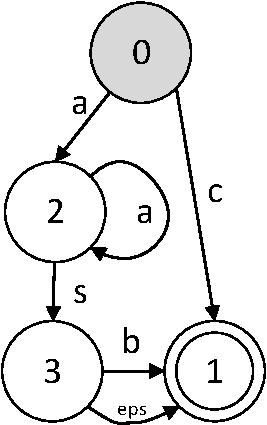
\includegraphics[scale=.6]{./Gorohov/pictures/G0initialAutomaton.pdf}
		\label{fig:initialAutomatonsForG0}
	}
	~
	\subfloat[Рекурсивный автомат $R_1$ для $G_1$]{
		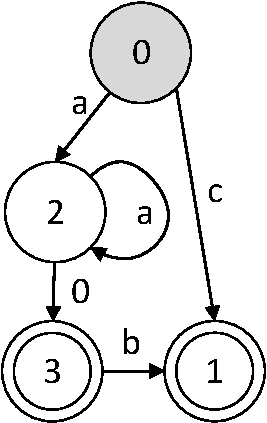
\includegraphics[scale=.6]{./Gorohov/pictures/G0minimizedAutomaton.pdf}
		\label{fig:RAForG0}
	}
	\caption{Преобразование грамматики в рекурсивный автомат}
	\label{fig:fig1}
\end{figure}

\subsection{Лес разбора для ECFG}
Результатом синтаксического анализа является структурное представление 
входа --- дерево или лес разбора в случае нескольких вариантов деревьев.
Для начала, определим дерево вывода для рекурсивного автомата: 
это дерево, корень которого помечен начальным состоянием, листья терминалы или $\varepsilon$,
а внутренние узлы нетерминалы N и их
дети образуют последовательность заданную путём в автомате, который начинается в 
состоянии $q_i$, где $ \Delta(q_i) = N $. Введём это определение более формально.

\begin{mydef}
	
	Дерево вывода последовательности $\alpha$ для рекурсивного автомата $R=(\Sigma, Q, S, F, \delta)$ это дерево со следующими свойствами:
	
	\begin{itemize}
		\item корень помечен $\Delta(S)$;
		\item листья --- терминалы $a\in (\Sigma \cup \varepsilon)$;
		\item остальные узлы --- нетерминалы $A\in \Delta(Q)$;
		\item у узла с меткой $N_i = \Delta(q_i)$ существует:
		\begin{itemize}
			\item 
			дети $l_0 \dots l_n (l_i \in \Sigma \cup \Delta(Q))$ тогда и только тогда,
			когда существует путь $p$ в $R$, $p = q_i \xrightarrow[]{l_0} q_{i+1} \xrightarrow[]{l_1} \dots \xrightarrow{l_n} q_m$, где
			$q_m \in F$, $l_i = 
			\left\{
			\begin{matrix}
			k_i, \text{ if } k_i \in \Sigma,\\
			\Delta(k_i), \text{ if } k_i \in Q,
			\end{matrix}
			\right.
			$
			\item только один ребенок помеченный $\varepsilon$ тогда и только тогда,
			когда $ q_i \in F $.
		\end{itemize}
	\end{itemize}
\end{mydef}
Для произвольных грамматик RA может быть неоднозначным с точки зрения допустимых путей,
поэтому можно получить несколько деревьев разбора для одной входной строки.
Shared Packed Parse Forest (SPPF)~\cite{SPPFa} может использоваться как компактное
представление всех возможных деревьев разбора. Будем использовать бинаризованную версию SPPF,
предложенную в~\cite{brnglr}, для уменьшения потребления памяти и достижения кубической
наихудшей временной и пространственной сложности. Бинаризованный SPPF может использоваться
в GLL~\cite{scott2013gll} и содержит следующие типы узлов (здесь i и j --- начало и конец выведенной подстроки во входной строке):

\begin{itemize}
	\item упакованные узлы вида $(S, k)$, где $S$ состояние автомата, k --- начало выведенной
	подстроки правого ребёнка; у упакованных узлов обязательно существует правый ребёнок ---
	символьный узел, и опциональный левый --- символьный или промежуточный узел;
	\item символьный узел помечен $(X, i, j)$ где $X \in \Sigma \cup \Delta(Q) \cup \{\varepsilon\}$;
	терминальные символьные узлы ($X \in \Sigma \cup \{\varepsilon\}$) --- листья;
	нетерминальные символьные узлы ($X \in \Delta(Q)$) могут иметь несколько упакованных детей;
	\item промежуточные узлы помечены $ (S, i, j) $, где $S$ состояние в автомате, могут иметь несколько упакованных детей.
\end{itemize}
Дети символьных и промежуточных узлов --- упакованные. Различные упакованные дети --- различные варианты поддеревьев.
Если у узла или его потомков более одного упакованного ребёнка, то он содержит несколько вариантов 
разбора для подстроки. Промежуточные и упакованные узлы необходимы для бинаризации SPPF, что обеспечивает большее переиспользование узлов.
Так, деревья, представленные на рис.~\ref{fig:Gtrees}, объединяются в SPPF показанный на рис.~\ref{fig:GSPPF}.
\begin{figure}
	\centering
	$
	\begin{array}[b]{rl}
	S ::= S\ S\ | \ c \ \ \ 
	\end{array}
	$
	\caption{Грамматика $G_0$}
	\label{fig:fig0}
\end{figure}
\begin{figure}[ht]   
	\centering
	\subfloat[Возможные деревья вывода]{
		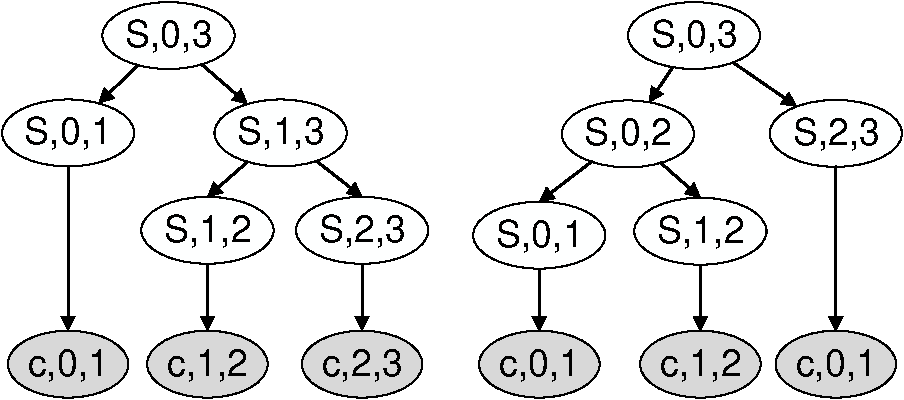
\includegraphics[scale=.3]{./Gorohov/pictures/Gtrees.pdf}
		\label{fig:Gtrees}
	}
	~
	\subfloat[SPPF]{
		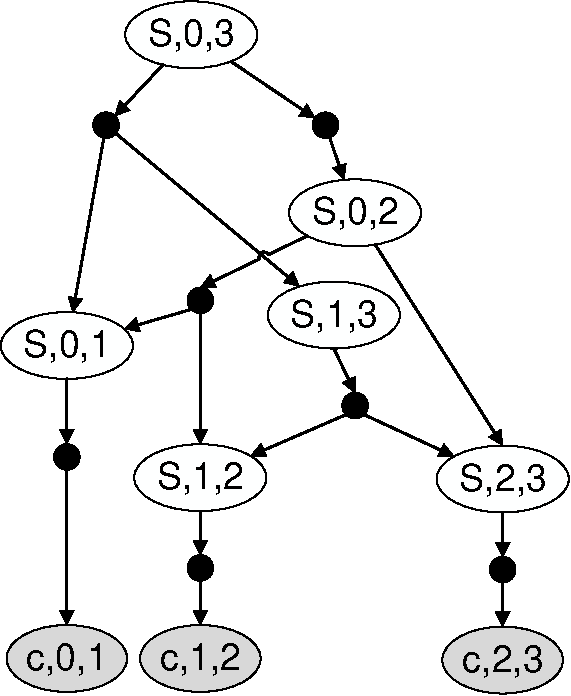
\includegraphics[scale=.3]{./Gorohov/pictures/GSPPF.pdf}
		\label{fig:GSPPF}
	}
	\caption{Пример для входа $ ccc $ и грамматики $G_0$}
	\label{fig:fig01}
\end{figure}
Опишем модификации исходных функций построения SPPF.
Функция \textbf{getNodeT$ (x, i) $}, которая создает терминальные узлы, 
повторно используется без каких-либо модификаций из базового алгоритма.
Чтобы обрабатывать недетерминизм в состояниях, определим функцию 
\textbf{getNodes}, которая проверяет, является ли следующее состояние RA финальным
и в этом случае строит нетерминальный узел в дополнение к промежуточному.
Она использует изменённую функцию \textbf{getNodeP}: вместо позиции в грамматики он 
принимает в качестве входных данных отдельно состояние RA и символ для нового узла SPPF:
текущий нетерминал или следующее состояние RA.

\begin{algorithmic}
\Function{getNodes}{$S, A, w, z$}
    \If{($S$ is final state)}
        \State $x \gets \textbf{getNodeP}(S, A, w, z)$
    \Else
        $\ x \gets \$ $
    \EndIf
    %\Statex
    %\If{$S.outedges = \varnothing$}
    %    \State $y \gets \$$
    %\Else
        \If{$(w = \$) \&$ not ($z$ is nonterminal node and its extents are equal)}
            \State $y \gets z$
        \Else
            $\ y \gets \textbf{getNodeP}(S, S, w, z)$
        \EndIf
    %\EndIf
    
    \State \Return{$(y,x)$}
\EndFunction   
\end{algorithmic}
\begin{algorithmic}
\Function{getNodeP}{$S, L, w, z$}
    \State $(\underline{\hspace{0.25cm}}, k, i) \gets z$
    
    \If{($w \neq \$$)}
        \State $(\underline{\hspace{0.25cm}}, j, k) \gets w$
    
        \State $y \gets$ find or create SPPF node labelled $(L, j, i)$  
    
        \If{($\nexists$ child of $y$ labelled $(S, k)$)}
            \State $y\prime \gets \textbf{new}$ $packedNode(S, k)$
            \State $y\prime.addLeftChild(w)$
            \State $y\prime.addRightChild(z)$
            \State $y.addChild(y\prime)$
        \EndIf
    
    \Else
        \State $y \gets$ find or create SPPF node labelled $(L, k, i)$ 
        \If{($\nexists$ child of $y$ labelled $(S, k)$)}
            \State $y\prime \gets \textbf{new}$ $packedNode(S, k)$
            \State $y\prime.addRightChild(z)$
            \State $y.addChild(y\prime)$
        \EndIf
    \EndIf
    \State \Return{$y$}
\EndFunction
\end{algorithmic}

Рассмотрим пример SPPF для ECFG $ G_1 $, показанные на рис.~\ref{fig:grammarG0}.
Эта грамматика содержит конструкции (условное вхождение (?) и повторение (+)),
которые должны быть преобразованы с использованием дополнительных нетерминалов 
для создания обычного GLL-анализатора.
Предложенный генератор строит рекурсивный автомат $ R_1 $~(рис.~\ref{fig:RAForG0})
и анализатор для него. Возможные деревья ввода последовательности $ aacb $ показаны 
на рис.~\ref{fig:treesForG0}. SPPF, созданный синтаксическим анализатором~(рис.~\ref{fig:SPPFForG0}),
содержит в себе все три дерева.

\begin{figure}[ht]   
	\centering
	\subfloat[Возможные деревья вывода]{
		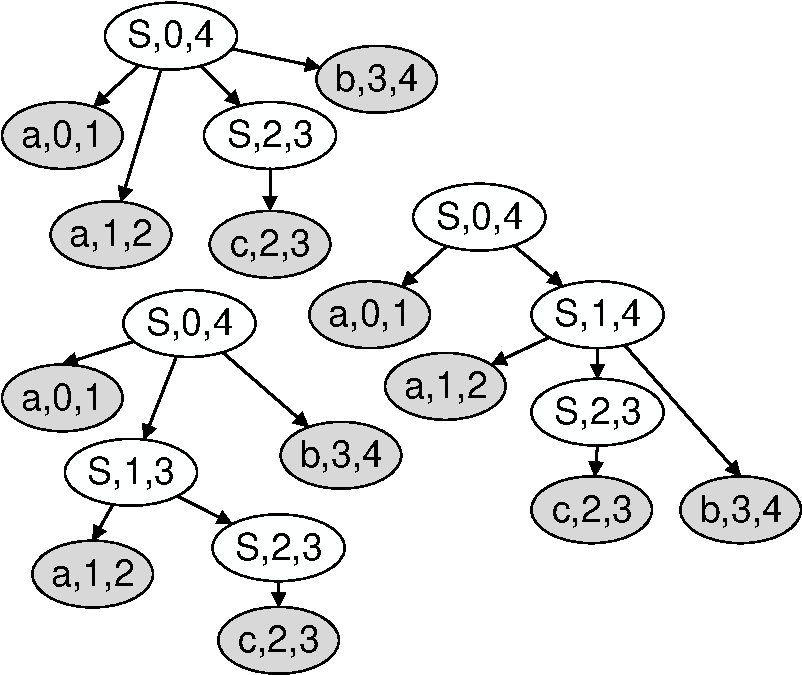
\includegraphics[scale=.4]{./Gorohov/pictures/G0trees.pdf}
		\label{fig:treesForG0}
	}
	~
	\subfloat[SPPF]{
		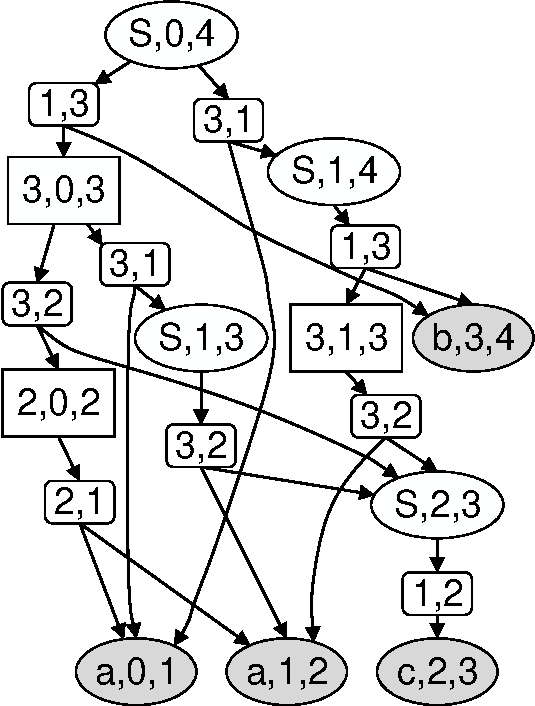
\includegraphics[scale=.4]{./Gorohov/pictures/G0SPPFwithPackedNodes.pdf}
		\label{fig:SPPFForG0}
	}
	\caption{Пример для входа $ aacb $ и автомата $R_1$}
	\label{fig:fig2}
\end{figure}

\subsection{Алгоритм построения леса разбора для ECFG}
В этом разделе описываются изменения в управляющих функциях базового алгоритма 
Generalised LL, необходимые для обработки ECFG. Основной цикл 
представленного алгоритма аналогичен базовому
GLL: на каждом шаге основная функция \textbf{parse} извлекает из очереди так называемый дескриптор
$R$ --- кортеж описывающий текущую ветку разбора. Пусть текущий дескриптор ($C_S, C_U, i, C_N$),
где $C_S$ --- состояние RA, $C_U$ --- узел GSS, i --- позицию во входной строке 
$\omega$, $C_N$ --- узел SPPF. В ходе обработки дескриптора могут возникнуть следующие
не исключающие друг друга ситуации.
\begin{itemize} 
	\item $C_S$ --- финальное состояние. Это возможно только если $C_S$
	--- стартовое состояние текущего нетерминала. Следует построить нетерминальный
	узел с ребёнком $(\varepsilon, i, i)$ и вызвать функцию \textbf{pop}, так как
	разбор нетерминала окончен.
	
	\item Существует терминальный переход $C_S \xrightarrow[]{\omega.[i]} q$.
	Во-первых, построить терминальный узел $ t = (\omega.[i], i, i+1) $, далее 
	вызвать функцию \textbf{getNodes} чтобы построить родителя для $ C_N $ и $ t $. 
	Функция \textbf{getNodes} возвращает кортеж $ (y, N) $, где $N$ --- опциональный
	нетерминальный узел. Создать дескриптор $ (q, C_U, i+1, y) $ и, если
	в $q$ ведёт несколько переходов, вызвать функцию \textbf{add} для этого дескриптора.
	Иначе поместить его в очередь вне зависимости от того был ли он создан до этого. 
	Если $ N \neq \$$,
	вызвать функцию \textbf{pop} для этого узла, состояния $ q $ и позиции во
	входе $ i + 1 $.
	
	\item Существуют нетерминальные переходы из $C_S$.
	Это значит, что следует начать разбор нового нетерминала, поэтому должен быть
	создан новый узел GSS, если такового ещё нет. Для этого нужно вызвать функцию
	\textbf{create} для каждого такого перехода. Она осуществляет необходимые
	операции с GSS и проверяет наличие узла GSS для текущих нетерминала и 
	позиции во входе.
\end{itemize}
Псевдокод для необходимых функций представлен ниже.

Функция \textbf{add} помещает в очередь дескриптор, если он не был создан до этого; эта функция не изменилась.
\begin{algorithmic}    
\Function{create}{$S_{call}, S_{next}, u, i, w$}
    \State $A \gets \Delta(S_{call})$
    \If{($\exists$ GSS node labeled $(A, i)$)}  
    
        \State $v \gets$ GSS node labeled $(A, i)$
        \If{(there is no GSS edge from $v$ to $u$ labeled ($S_{next},w$))}
            \State add GSS edge from $v$ to $u$ labeled ($S_{next},w$)
            \For{($(v, z) \in \mathcal{P} $)}
                \State $(y,N) \gets$ \textbf{getNodes}($S_{next}, u.nonterm, w, z$)
                
                \State $(\_, \_, h) \gets y$
                \State \textbf{add}($S_{next} , u, h, y$)
                
                \If{$N \neq \$$}
                    \State $(\_, \_, h) \gets N$;
                    \textbf{pop}$(u,h,N)$ 
                \EndIf
            \EndFor
        \EndIf
    \Else
        \State $v \gets$ \textbf{new} GSS node labeled $(A, i)$
        \State create GSS edge from $v$ to $u$ labeled ($S_{next}, w$)
        \State \textbf{add}($S_{call}, v, i, \$ $)
    \EndIf
    \Return{$v$}
\EndFunction
\end{algorithmic}  

\begin{algorithmic}   
\Function{pop}{$u,i,z$}
    \If{($(u,z) \notin \mathcal{P}$)}  
        \State $\mathcal{P}.add(u,z)$
        \ForAll{GSS edges $(u,S,w,v)$}
            \State $(y,N) \gets$ \textbf{getNodes}($S, v.nonterm, w, z$)
            \State \textbf{add}($S,v,i,y$)
            \If{$N \neq \$$}
                \ \textbf{pop}$(v,i,N)$ 
            \EndIf
        \EndFor
    \EndIf
\EndFunction
\end{algorithmic}

%\textbf{Pop} function is called when we reach final state. It queues descriptors for all outgoing edges from current GSS node.

\begin{algorithmic}
\Function{parse}{}
    \State $GSSroot\gets new GSSnode(StartNonterminal,0) $
    \State $R.enqueue(StartState, GSSroot, 0, \$)$
    \While{$R \neq \varnothing $}
    \State{$(C_{S},C_{U},i,C_{N}) \gets R.dequeue()$}
    
    \If{ ($C_{N} = \$ $) and ($C_{S}$ is final state)}
    \State $eps \gets \textbf{getNodeT}(\varepsilon, i)$  
    \State $(\underline{\hspace{0.25cm}}, N) \gets \textbf{getNodes}(C_{S},C_{U}.nonterm, \$, eps)$
    \State \textbf{pop}$(C_{U},i,N)$ 
    \EndIf
    
    \For{\textbf{each} $transition (C_{S},label,S_{next})$}
        \Switch{$label$}  
        \Case{$Terminal(x)$ where ($x = input[i]$)}
            \State $T \gets \textbf{getNodeT}(x, i)$
            
            \State $(y, N) \gets \textbf{getNodes}(S_{next},C_{U}.nonterm, C_{N}, T)$
            \If{$N \neq \$$}
                \ \textbf{pop}$(C_{U},i+1,N)$ 
            \EndIf
            
            \If{$S_{next}$ has multiple ingoing transitions}
            \State $\textbf{add}(S_{next}, C_{U}, i + 1, y)$
            \Else
            \State $R.enqueue(S_{next}, C_{U}, i + 1, y)$
            \EndIf
        \EndCase
    
        \Case{$Nonterminal(S_{call})$}
    %\State{$slots \gets pTable[A][input[i]]$}
    %\If{$slots \neq \varnothing$}
            \State \textbf{create}($S_{call}, S_{next}, C_{U}, i, C_{N}$)
    %\EndIf
    %\ForAll{$L \in slots$}
    %    \State{\Call{add}{L,u,i,\$}} 
    %\EndFor
        \EndCase
        \EndSwitch
        
    \EndFor
    \EndWhile
    \If{SPPF node ($StartNonterminal,0,input.length$) exists}
    \State return this node
    \Else
    \ report failure
    \EndIf
\EndFunction
\end{algorithmic}




\section{Синтаксический анализ регулярных множеств}

Описанный в данной работе алгоритм можно применять для анализа регулярных множеств.
При работе с конечным автоматом в качестве входных данных необходимо обрабатывать все переходы из текущей позиции (состояния) в автомате.
Так, основная функция приобретает следующий вид:
\begin{algorithmic}
\Function{parseRegularSet}{}
    \State $GSSroot\gets new GSSnode(StartNonterminal,StartState) $
    \State $R.enqueue(StartState, GSSroot, StartState, \$)$
    \While{$R \neq \varnothing $}
    \State{$(C_{S},C_{U},i,C_{N}) \gets R.dequeue()$}
    
    \If{ ($C_{N} = \$ $) and ($C_{S}$ is final state)}
    \State $eps \gets \textbf{getNodeT}(\varepsilon, i)$  
    \State $(\underline{\hspace{0.25cm}}, N) \gets \textbf{getNodes}(C_{S},C_{U}.nonterm, \$, eps)$
    \State \textbf{pop}$(C_{U},i,N)$
    \EndIf
    
    \For{\textbf{each} $transition (C_{S},label,S_{next})$}
        \Switch{$label$}
        \Case{$Terminal(x)$}
            \For{\textbf{each} (input[i] $\xrightarrow[]{x}$ input[k])}
            \State $T \gets \textbf{getNodeT}(x, i)$
            
            \State $(y, N) \gets \textbf{getNodes}(S_{next},C_{U}.nonterm, C_{N}, T)$
            \If{$N \neq \$$}
                \ \textbf{pop}$(C_{U},k,N)$ 
            \EndIf
            
            %\If{$S_{next}$ have multiple ingoing transitions}
            \State $\textbf{add}(S_{next}, C_{U}, k, y)$
            %\Else
            %\State $R.enqueue(S_{next}, C_{U}, k, y)$
            %\State $\textbf{add}(S_{next}, C_{U}, k, y)$
            %\EndIf
            \EndFor
        \EndCase
    
        \Case{$Nonterminal(S_{call})$}
    %\State{$slots \gets pTable[A][input[i]]$}
    %\If{$slots \neq \varnothing$}
            \State \textbf{create}($S_{call}, S_{next}, C_{U}, i, C_{N}$)
    %\EndIf
    %\ForAll{$L \in slots$}
    %    \State{\Call{add}{L,u,i,\$}} 
    %\EndFor
        \EndCase
        \EndSwitch
        
    \EndFor
    \EndWhile
    \If{SPPF node ($StartNonterminal,StartState,\_$) exists}
    \State return this node
    \Else
    \ report failure
    \EndIf
\EndFunction
\end{algorithmic}
Позициями во входе для автомата становятся номера состояний и обрабатываются все исходящие переходы во входе. Кроме того,    
Функция \textbf{add} вызывается при обработке терминального перехода всегда, чтобы поддержать возможные циклы во входе.
Например, для грамматики $S ::= a*$ и входного автомата на рис.~\ref{graphEx}
дескриптор будет создаваться бесконечно, если не добавить его в множество созданных, и алгоритм не остановится.
Данное изменение не меняет теоретическую сложность алгоритма, но может сказаться на производительности в худшую сторону.
Поэтому этот подход можно применять лишь только в случае присутствия циклов во ходе, иначе вызывать функцию \textbf{add}
только при наличии нескольких входящих переходов в текущее состояние.

\begin{figure}%[ht]   
	\centering
	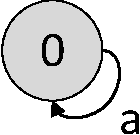
\includegraphics[scale=.5]{./Gorohov/pictures/graphEx.pdf}
	\caption{Пример входа для грамматики $S ::= a^*$.}
	\label{graphEx}
\end{figure}

\section{Эксперименты}
В работе~\cite{scott2016structuring}
было проведено экспериментальное сравнение алгоритма для факторизованных грамматик (Factorised GLL, FGLL) и базового GLL-алгоритма,
продемонстрировавшее, что FGLL показывает большую производительность для грамматик в форме Бэкуса-Наура, которые могут быть факторизованы.
Предполагается, что предложенная в данной работе версия алгоритма
продемонстрирует большую производительность, чем FGLL, для грамматик, имеющих эквивалентные позиции для алгоритма минимизации автомата,
но различные после факторизации. Автомат, построенный для грамматики, в которой есть эквивалентные позиции, для которых алгоритм создаёт большое количество дескрипторов,
объединит данные позиции, сократив тем самым множество создаваемых дескрипторов,
что в свою очередь увеличит производительность. Примером такой ситуации может служить грамматика 
$G_2$~(рис.~\ref{fig:grammarG1}), так как она содержит длинные последовательности 
в альтернативах, которые не сливаются при факторизации, но эквивалентны для алгоритма минимизации автомата.
Рекурсивный автомат построенный для этой грамматики показан на рис.~\ref{fig:automatonForG1}.

\begin{figure}[ht]   
	\centering
	\subfloat[Грамматика $G_2$]{
		$
		\begin{array}{rl}
		S ::=& K\ (K\ K\ K\ K\ K \ |\ a\ K\ K\ K\ K) \\
		K ::=& S\ K\ |\ a\ K\ |\ a \\
		\end{array}
		$
		\label{fig:grammarG1}
	}
	
	\subfloat[Рекурсивный автомат для грамматики $G_2$]{
		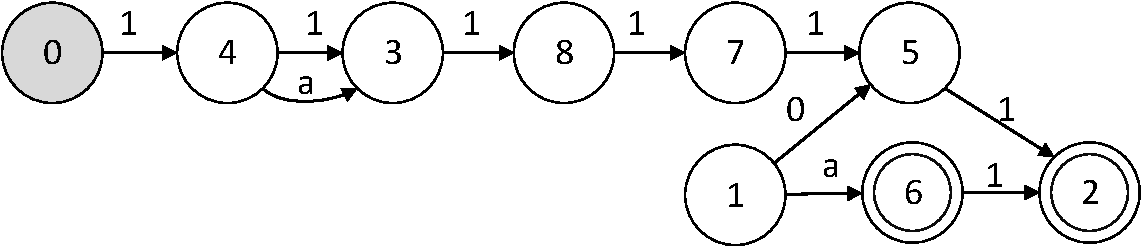
\includegraphics[scale=.5]{./Gorohov/pictures/G1automaton.pdf}
		\label{fig:automatonForG1}
	}
	\caption{Грамматика $G_2$ и RA для неё}
\end{figure}

Эксперименты проводились на входах различной длины, результаты приведены на рис.~\ref{expPlots}.
Точные данные для входа $a^{450}$ показаны в таблице~\ref{expTable}.

Для экспериментов использовался ПК со следующими характеристиками: Microsoft Windows 10 Pro x64, Intel(R) Core(TM) i7-4790 
CPU @ 3.60GHz, 3601 Mhz, 4 Cores, 4 Logical Processors, 16 GB.

\begin{figure}
    \centering
    \subfloat[Количество рёбер GSS.]{
        \begin{tikzpicture}[scale=.5]
        \begin{axis}[
        legend cell align=left,
        legend pos = north west,
        xlabel = {Длина входа},
        ylabel = {Рёбра GSS},
        %ymode=log
        ]
        \addplot [only marks, mark=triangle*] coordinates {
            (30,4022) (60,17012) (90,39002) (120,69992) (150,109982) (180,158972) (210,216962) (240,283952) (270,359942) (300,444932) (330,538922) (360,641912) (390,753902) (420,874892) (450,1004882)
        };
        \addplot [only marks, mark=*] coordinates {
            (30,2452) (60,10282) (90,23512) (120,42142) (150,66172) (180,95602) (210,130432) (240,170662) (270,216292) (300,267322) (330,323752) (360,385582) (390,452812) (420,525442) (450,603472)
        };
        \legend{ 
            Грамматика, 
            Автомат
        };
        \end{axis}
        \end{tikzpicture}
        \label{fig:GSSedges}
    }
    ~
    \subfloat[Время работы.]{
        \begin{tikzpicture}[scale=.5]
        \begin{axis}[
        legend cell align=left,
        legend pos = north west,
        xlabel = {Длина входа},
        ylabel = {Время, с},
        %ymode=log
        ]
        \addplot [only marks, mark=triangle*] coordinates {
            (30,00.1690245) (60,01.1310924) (90,03.6899218) (120,11.1006359) (150,20.8163584) (180,28.7973458) (210,45.3640866) (240,68.3269546) (270,102.2953852) (300,150.2681210) (330,197.9508999) (360,269.1387530) (390,346.4999998) (420,442.0947044) (450,613.3386222)
        };
        \addplot [only marks, mark=*] coordinates {
            (30,00.0625041) (60,00.6562026) (90,02.6719009) (120,04.3594156) (150,09.2969549) (180,15.6406979) (210,25.3438039) (240,39.1251338) (270,57.6720586) (300,82.0470354) (330,109.7031754) (360,150.5466896) (390,191.5317906) (420,241.1571067) (450,351.8283519)
        };
        \legend{ 
            Грамматика, 
            Автомат
        };
        \end{axis}
        \end{tikzpicture}
        \label{fig:Time}
    }

    \subfloat[Количество узлов SPPF.]{
        \begin{tikzpicture}[scale=.5]
        \begin{axis}[
        legend cell align=left,
        legend pos = north west,
        xlabel = {Длина входа},
        ylabel = {Узлы SPPF},
        %ymode=log
        ]
        \addplot [only marks, mark=triangle*] coordinates {
            (30,49430) (60,429210) (90,1490290) (120,3583670) (150,7060350) (180,12271330) (210,19567610) (240,29300190) (270,41820070) (300,57478250) (330,76625730) (360,99613510) (390,126792590) (420,158513970) (450,195128650)
        };
        \addplot [only marks, mark=*] coordinates {
            (30,30695) (60,264835) (90,918375) (120,2207315) (150,4347655) (180,7555395) (210,12046535) (240,18037075) (270,25743015) (300,35380355) (330,47165095) (360,61313235) (390,78040775) (420,97563715) (450,120098055)
        };
        \legend{ 
            Грамматика, 
            Автомат
        };
        \end{axis}
        \end{tikzpicture}
        \label{fig:SPPFnodes}
    }
    ~
    \subfloat[Использование памяти]{
        \begin{tikzpicture}[scale=.5]
        \begin{axis}[
        legend cell align=left,
        legend pos = north west,
        xlabel = {Длина входа},
        ylabel = {Память, Мб},
        %ymode=log
        ]
        \addplot [only marks, mark=triangle*] coordinates {
             (90,130) (120,267) (150,491) (180,842) (210,1318) (240,1977) (270,2827) (300,3869) (330,5183) (360,6665) (390,8583) (420,10671) (450,11818)
        };
        \addplot [only marks, mark=*] coordinates {
            (90,106) (120,190) (150,325) (180,531) (210,829) (240,1225) (270,1728) (300,2359) (330,3161) (360,4126) (390,5242) (420,6571) (450,8026)
        };
        \legend{ 
            Грамматика, 
            Автомат
        };
        \end{axis}
        \end{tikzpicture}
        \label{fig:Memory}
    }
    
    \subfloat[Количество дескрипторов.]{
        \begin{tikzpicture}[scale=.5]
        \begin{axis}[
        legend cell align=left,
        legend pos = north west,
        xlabel = {Длина входа},
        ylabel = {Дескрипторы},
        %ymode=log
        ]
        \addplot [only marks, mark=triangle*] coordinates {
            (30,4346) (60,18551) (90,42656) (120,76661) (150,120566) (180,174371) (210,238076) (240,311681) (270,395186) (300,488591) (330,591896) (360,705101) (390,828206) (420,961211) (450,1104116)
        };
        \addplot [only marks, mark=*] coordinates {
            (30,3181) (60,13531) (90,31081) (120,55831) (150,87781) (180,126931) (210,173281) (240,226831) (270,287581) (300,355531) (330,430681) (360,513031) (390,602581) (420,699331) (450,803281)
        };
        \legend{ 
            Грамматика, 
            Автомат
        };
        \end{axis}
        \end{tikzpicture}
        \label{fig:Descriptors}
    }
    \caption{Результаты экспериментов с грамматикой $G_2$.}
    \label{expPlots}
\end{figure}

\begin{table}[ht]   
	\begin{center}
		\begin{tabular}{ | c | c | c | c | c | c | c |  }
			\hline
			& \rotatebox[origin=c]{90}{Время}
			& \rotatebox[origin=c]{90}{Дескрипторы} &
			\rotatebox[origin=c]{90}{Рёбра GSS} &
			\rotatebox[origin=c]{90}{Узлы GSS} &
			\rotatebox[origin=c]{90}{Узлы SPPF} &
			\rotatebox[origin=c]{90}{Память, Мб} \\ \hline
			FGLL & 10 мин. 13 с.  & 1104116        & 1004882      & 902        & 195 млн. &  11818 \\ \hline 
			RA       & 5 мин. 51 с.  & 803281        & 603472      & 902        & 120 млн. & 8026  \\ \hline \hline
			Ratio   &  43$\%$       & 28$\%$     & 40 $\%$    &  0 $\%$ &  39 $\%$ &  33 $\%$ \\ \hline
		\end{tabular}
	\end{center}
	\caption{Результаты экспериментов для входа $a^{450}$}
	\label{expTable}
\end{table}

Результаты данных экспериментов поддерживают предположение о том, что на некоторых грамматиках 
предложенный подход показывает результаты лучше FGLL.
Для этого рекурсивного автомата анализатор создаёт меньше дескрипторов, чем для грамматики, так как 
цепочки нетерминалов $K$ в альтернативах представлены единственным путём в автомате. Эта особенность ведёт к снижению количества 
узлов SPPF и размера GSS.
В среднем, с грамматикой $G_2$ версия с минимизированными автоматами работает на $43\%$ быстрее,
использует на $28\%$ меньше дескрипторов, на $40\%$ меньше рёбер GSS, создаёт на $39\%$ меньше узлов SPPF
и использует на $33\%$ меньше памяти.

Было проведено экспериментальное сравнение разработанного алгоритма GLL с
существующим в проекте YaccConstructor (основан на оригинальном алгоритме Generalised LL) в задаче поиска 16s рРНК в метагеномной сборке.
Длинные рёбра сборки были предварительно отфильтрованы с помощью инструмента Infernal.
В результате фильтрации сборка разбивается на компоненты, которые можно анализировать независимо друг от
друга. Тем не менее, предложенный ранее алгоритм не позволяет обработать некоторые компоненты, поэтому сравнение проводилось
на остальных: 10 компонент с 400-100 состояний и переходов и 1118 компонент с менее чем 100 состояний и переходов.
Результаты сравнения приведены в таблице~\ref{expTable1} и показывают, что при работе с метагеномными сборками новый
алгоритм, в среднем, использует на 65\% меньше памяти и работает на 45\% быстрее базового GLL. Сравнение с FGLL
показывает на 4\% меньшее использование памяти новым алгоритмом и на 10\% меньшее время работы.

\begin{table}
	\begin{center}
		\begin{tabular}{ | c | c | c | c | c | c |}
			\hline
			& &\multicolumn{2}{c|}{GSS} & & \\
			\cline{3-4}
			& Деск-ры & Рёбра   & Узлы   & Память& Время   \\ \hline
			GLL               &  802млн &  414млн & 339млн  & 20Гб & 52 мин. 43 с.  \\ \hline
			FGLL        &  382млн &  187млн & 134млн & 7Гб & 29 мин. 27 с.  \\ \hline
			RA                &  362млн &  190млн & 134млн & 6,8Гб & 26 мин. 34 с.  \\ \hline %\hline
			%Ratio   &  9$\%$       & 13$\%$     & 12 $\%$    &  3 $\%$  & 14 $\%$\\ \hline
		\end{tabular}
		\caption{Результаты экспериментов с метагеномной сборкой}
		\label{expTable1}
	\end{center}
\end{table}

\section*{Заключение}
В рамках данной работы была разработана и реализована модификация алгоритма GLL,
работающая с расширенными контекстно-свободными грамматиками. Показано, что полученный
алгоритм повышает производительность поиска структур, заданных с помощью контекстно-свободной
грамматики в метагеномных сборках. Описанный алгоритм и генератор синтаксических анализаторов реализованы
в расках проекта YaccConstructor на языке программирования F\#.
Исходный код доступен в репозитории проекта:~\url{https://github.com/YaccConstructor/YaccConstructor}.

Одним из методов для описания семантики языка являются атрибутные грамматики, но они не поддержаны в описанном алгоритме.
Опубликовано несколько работ о подклассе атрибутных ECFG (например~\cite{AttributedELL}), тем не менее нет общего решения для произвольных ECFG.
Таким образом, поддержка атрибутных расширенных контекстно-свободных грамматик и подсчёт семантики может быть дальнейшим развитием данной работы.
%\setmonofont[Mapping=tex-text]{CMU Typewriter Text}
%\bibliographystyle{ugost2008ls}
\begin{thebibliography}{10}
	\def\selectlanguageifdefined#1{
		\expandafter\ifx\csname date#1\endcsname\relax
		\else\selectlanguage{#1}\fi}
	\providecommand*{\href}[2]{{\small #2}}
	\providecommand*{\url}[1]{{\small #1}}
	\providecommand*{\BibUrl}[1]{\url{#1}}
	\providecommand{\BibAnnote}[1]{}
	\providecommand*{\BibEmph}[1]{#1}
	\ProvideTextCommandDefault{\cyrdash}{\iflanguage{russian}{\hbox
			to.8em{--\hss--}}{\textemdash}}
	\providecommand*{\BibDash}{\ifdim\lastskip>0pt\unskip\nobreak\hskip.2em plus
		0.1em\fi
		\cyrdash\hskip.2em plus 0.1em\ignorespaces}
	\renewcommand{\newblock}{\ignorespaces}
	
	\bibitem{ANTLRa}
	\selectlanguageifdefined{english}
	ANTLR Project website. \BibDash
	\newblock \url{http://www.antlr.org/}.
	
	\bibitem{afroozeh2015faster}
	\selectlanguageifdefined{english}
	\BibEmph{Afroozeh~Ali, Izmaylova~Anastasia}. Faster, Practical {GLL} Parsing~//
	International Conference on Compiler Construction~/ Springer. \BibDash
	\newblock 2015. \BibDash
	\newblock P.~89--108.
	
	\bibitem{aho1974design}
	\selectlanguageifdefined{english}
	\BibEmph{Aho~Alfred~V, Hopcroft~John~E}. The design and analysis of computer
	algorithms. \BibDash
	\newblock Pearson Education India, 1974.
	
	\bibitem{AttributedELL}
	\selectlanguageifdefined{english}
	\BibEmph{Alblas~Henk, Schaap-Kruseman~Joos}. An attributed {ELL} (1)-parser
	generator~// International Workshop on Compiler Construction~/ Springer.
	\BibDash
	\newblock 1990. \BibDash
	\newblock P.~208--209.
	
	\bibitem{Bison}
	\selectlanguageifdefined{english}
	Bison Project website. \BibDash
	\newblock \url{https://www.gnu.org/software/bison/}.
	
	\bibitem{Breveglieri2014}
	\selectlanguageifdefined{english}
	\BibEmph{Breveglieri~Luca, Crespi~Reghizzi~Stefano, Morzenti~Angelo}.
	\href{http://dx.doi.org/10.1007/978-3-319-04921-2_18}{Shift-Reduce Parsers
		for Transition Networks}~// Language and Automata Theory and Applications:
	8th International Conference, LATA 2014, Madrid, Spain, March 10-14, 2014.
	Proceedings~/ Ed.\ by\ Adrian-Horia~Dediu, Carlos~Mart{\'i}n-Vide,
	Jos{\'e}-Luis~Sierra-Rodr{\'i}guez, Bianca~Truthe. \BibDash
	\newblock Cham~: Springer International Publishing, 2014. \BibDash
	\newblock P.~222--235. \BibDash
	\newblock
	ISBN:~\href{http://isbndb.com/search-all.html?kw=978-3-319-04921-2}{978-3-319-04921-2}.
	\BibDash
	\newblock Access mode: \BibUrl{http://dx.doi.org/10.1007/978-3-319-04921-2_18}.
	
	\bibitem{ELRR}
	\selectlanguageifdefined{english}
	\BibEmph{Breveglieri~Luca, Reghizzi~Stefano~Crespi, Morzenti~Angelo}.
	Shift-reduce parsers for transition networks~// International Conference on
	Language and Automata Theory and Applications~/ Springer. \BibDash
	\newblock 2014. \BibDash
	\newblock P.~222--235.
	
	\bibitem{PredictiveECFG}
	\selectlanguageifdefined{english}
	\BibEmph{Br{\"u}ggemann-Klein~Anne, Wood~Derick}. On predictive parsing and
	extended context-free grammars~// International Conference on Implementation
	and Application of Automata~/ Springer. \BibDash
	\newblock 2002. \BibDash
	\newblock P.~239--247.
	
	\bibitem{ECFGparsing}
	\selectlanguageifdefined{english}
	\BibEmph{Bruggemann-Klein~Anne, Wood~Derick}. The parsing of extended
	context-free grammars. \BibDash
	\newblock 2002.
	
	\bibitem{ELLParser}
	\selectlanguageifdefined{english}
	\BibEmph{Heckmann~Reinhold}. An efficient {ELL} (1)-parser generator~//
	\BibEmph{Acta Informatica}. \BibDash
	\newblock 1986. \BibDash
	\newblock Vol.~23, no.~2. \BibDash
	\newblock P.~127--148.
	
	\bibitem{ELL}
	\selectlanguageifdefined{english}
	\BibEmph{Heilbrunner~Stephan}. On the definition of {ELR} (k) and ELL (k)
	grammars~// \BibEmph{Acta Informatica}. \BibDash
	\newblock 1979. \BibDash
	\newblock Vol.~11, no.~2. \BibDash
	\newblock P.~169--176.
	
	\bibitem{ECFG}
	\selectlanguageifdefined{english}
	\BibEmph{Hemerik~Kees}. Towards a Taxonomy for {ECFG} and {RRPG} Parsing~//
	International Conference on Language and Automata Theory and Applications~/
	Springer. \BibDash
	\newblock 2009. \BibDash
	\newblock P.~410--421.
	
	\bibitem{hopcroft1971n}
	\selectlanguageifdefined{english}
	An n log n algorithm for minimizing states in a finite automaton~: Rep.~/ DTIC
	Document~; Executor: John~Hopcroft~: 1971.
	
	\bibitem{lee1997characterization}
	\selectlanguageifdefined{english}
	\BibEmph{Lee~Gyung-Ok, Kim~Do-Hyung}. Characterization of extended LR (k)
	grammars~// \BibEmph{Information processing letters}. \BibDash
	\newblock 1997. \BibDash
	\newblock Vol.~64, no.~2. \BibDash
	\newblock P.~75--82.
	
	\bibitem{ELALR}
	\selectlanguageifdefined{english}
	\BibEmph{Morimoto~Shin-ichi, Sassa~Masataka}. Yet another generation of {LALR}
	parsers for regular right part grammars~// \BibEmph{Acta informatica}.
	\BibDash
	\newblock 2001. \BibDash
	\newblock Vol.~37, no.~9. \BibDash
	\newblock P.~671--697.
	
	\bibitem{Infernal}
	\selectlanguageifdefined{english}
	\BibEmph{Nawrocki~Eric~P, Eddy~Sean~R}. Infernal 1.1: 100-fold faster RNA
	homology searches~// \BibEmph{Bioinformatics}. \BibDash
	\newblock 2013. \BibDash
	\newblock Vol.~29, no.~22. \BibDash
	\newblock P.~2933--2935.
	
	\bibitem{ELRParsing}
	\selectlanguageifdefined{english}
	\BibEmph{Purdom~Jr~Paul~Walton, Brown~Cynthia~A}. Parsing extended {LR} (k)
	grammars~// \BibEmph{Acta Informatica}. \BibDash
	\newblock 1981. \BibDash
	\newblock Vol.~15, no.~2. \BibDash
	\newblock P.~115--127.
	
	\bibitem{Anderson2013a}
	\selectlanguageifdefined{english}
	Quantifying variances in comparative RNA secondary structure prediction~/
	James~WJ~Anderson, {\'A}d{\'a}m~Nov{\'a}k, Zsuzsanna~S{\"u}k{\"o}sd et~al.~//
	\href{http://dx.doi.org/10.1186/1471-2105-14-149}{\BibEmph{BMC
			Bioinformatics}}. \BibDash
	\newblock 2013. \BibDash
	\newblock Vol.~14, no.~1. \BibDash
	\newblock P.~149.
	
	\bibitem{ragozina}
	\selectlanguageifdefined{english}
	\BibEmph{Ragozina~Anastasiya}. {GLL}-based relaxed parsing of dynamically
	generated code~: Master’s Thesis~/ Anastasiya~Ragozina~; SpBU. \BibDash
	\newblock 2016.
	
	\bibitem{reago}
	\selectlanguageifdefined{english}
	Reconstructing 16S rRNA genes in metagenomic data~/ Cheng~Yuan, Jikai~Lei,
	James~Cole, Yanni~Sun~// \BibEmph{Bioinformatics}. \BibDash
	\newblock 2015. \BibDash
	\newblock Vol.~31, no.~12. \BibDash
	\newblock P.~i35--i43.
	
	\bibitem{SPPFa}
	\selectlanguageifdefined{english}
	\BibEmph{Rekers~Joan~Gerard}. Parser generation for interactive environments~:
	Ph.\,D. thesis~/ Joan~Gerard~Rekers~; Universiteit van Amsterdam. \BibDash
	\newblock 1992.
	
	\bibitem{scott2010gll}
	\selectlanguageifdefined{english}
	\BibEmph{Scott~Elizabeth, Johnstone~Adrian}. {GLL} parsing~//
	\BibEmph{Electronic Notes in Theoretical Computer Science}. \BibDash
	\newblock 2010. \BibDash
	\newblock Vol. 253, no.~7. \BibDash
	\newblock P.~177--189.
	
	\bibitem{scott2013gll}
	\selectlanguageifdefined{english}
	\BibEmph{Scott~Elizabeth, Johnstone~Adrian}. {GLL} parse-tree generation~//
	\BibEmph{Science of Computer Programming}. \BibDash
	\newblock 2013. \BibDash
	\newblock Vol.~78, no.~10. \BibDash
	\newblock P.~1828--1844.
	
	\bibitem{scott2016structuring}
	\selectlanguageifdefined{english}
	\BibEmph{Scott~Elizabeth, Johnstone~Adrian}. Structuring the {GLL} parsing
	algorithm for performance~// \BibEmph{Science of Computer Programming}.
	\BibDash
	\newblock 2016. \BibDash
	\newblock Vol. 125. \BibDash
	\newblock P.~1--22.
	
	\bibitem{brnglr}
	\selectlanguageifdefined{english}
	\BibEmph{Scott~Elizabeth, Johnstone~Adrian, Economopoulos~Rob}. {BRNGLR}: a
	cubic Tomita-style {GLR} parsing algorithm~// \BibEmph{Acta informatica}.
	\BibDash
	\newblock 2007. \BibDash
	\newblock Vol.~44, no.~6. \BibDash
	\newblock P.~427--461.
	
	\bibitem{tellier2006learning}
	\selectlanguageifdefined{english}
	\BibEmph{Tellier~Isabelle}. Learning recursive automata from positive
	examples~// \BibEmph{Revue des Sciences et Technologies de
		l'Information-S{\'e}rie RIA: Revue d'Intelligence Artificielle}. \BibDash
	\newblock 2006. \BibDash
	\newblock Vol.~20, no.~6. \BibDash
	\newblock P.~775--804.
	
	\bibitem{Thompson:1968:PTR:363347.363387}
	\selectlanguageifdefined{english}
	\BibEmph{Thompson~Ken}. Programming Techniques: Regular Expression Search
	Algorithm~// \href{http://dx.doi.org/10.1145/363347.363387}{\BibEmph{Commun.
			ACM}}. \BibDash
	\newblock 1968. \BibDash Jun. \BibDash
	\newblock Vol.~11, no.~6. \BibDash
	\newblock P.~419--422. \BibDash
	\newblock Access mode: \BibUrl{http://doi.acm.org/10.1145/363347.363387}.
	
	\bibitem{hmmer}
	\selectlanguageifdefined{english}
	\BibEmph{Wheeler~Travis~J, Eddy~Sean~R}. nhmmer: DNA homology search with
	profile HMMs~// \BibEmph{Bioinformatics}. \BibDash
	\newblock 2013. \BibDash
	\newblock P.~btt403.
	
	\bibitem{EBNFISO}
	\selectlanguageifdefined{english}
	\BibEmph{Wirth~Niklaus}. Extended Backus-Naur Form ({EBNF})~//
	\BibEmph{ISO/IEC}. \BibDash
	\newblock 1996. \BibDash
	\newblock Vol. 14977. \BibDash
	\newblock P.~2996.
	
	\bibitem{xander}
	\selectlanguageifdefined{english}
	Xander: employing a novel method for efficient gene-targeted metagenomic
	assembly~/ Qiong~Wang, Jordan~A.~Fish, Mariah~Gilman et~al.~//
	\href{http://dx.doi.org/10.1186/s40168-015-0093-6}{\BibEmph{Microbiome}}.
	\BibDash
	\newblock 2015. \BibDash
	\newblock Vol.~3, no.~1. \BibDash
	\newblock P.~32. \BibDash
	\newblock Access mode: \BibUrl{http://dx.doi.org/10.1186/s40168-015-0093-6}.
	
	\bibitem{YaccConstructor}
	\selectlanguageifdefined{russian}
	YaccConstructor [Электронный ресурс]. \BibDash
	\newblock {Режим доступа}:
	\BibUrl{https://github.com/YaccConstructor/YaccConstructor} ({дата обращения}:
	11.05.2015).
	
\end{thebibliography}


